\apendice{Especificación de Requisitos}

\section{Introducción}

En esta sección se hace referencia a los requerimientos que debe cumplir el software para satisfacer las necesidades del cliente e identificar los componentes necesarios para entregar un producto adecuado. 


\section{Objetivos generales}

A lo largo de la memoria ya se han definido distintos objetivos del proyecto, pero estos pueden ser resumidos en los siguientes puntos:

\begin{itemize}

\item \textbf{Tecnología \textit{blockchain}:} Uso de la tecnología \textit{blockchain} como base para la creación de un sistema de contratación descentralizado y seguro.
Se busca garantizar la transparencia e inmutabilidad de los datos, permitiendo que todas las transacciones queden registradas de forma segura.

\item \textbf{Contratos Inteligentes:} Desarrollo de contratos inteligentes que aseguraran el cumplimiento de acuerdos laborales.
Estos contratos deben de ser capaz de autoejecutarse en función de las condiciones preestablecidas por las partes. El principal objetivo es reducir la necesidad de intermediarios.

\item \textbf{Identificación segura mediante dispositivo móvil:} Implementación de métodos de autenticación y verificación seguros utilizando dispositivos móviles, como biometría o códigos QR.
Se pretende asegurar que solo los usuarios autorizados puedan acceder a un contrato y realizar operaciones dentro del sistema.

\item \textbf{Desarrollo de Aplicación Móvil:} Creación de una aplicación móvil Android que sirva de interfaz para interactuar con los contratos inteligentes y la \textit{blockchain}, escondiendo toda la complejidad al usuario.
La aplicación debe de estar diseñada para ser intuitiva, con el objetivo de que sea fácilmente utilizable para personas con cualquier nivel de habilidades tecnológicas.

\end{itemize}

\section{Catálogo de requisitos}

En este apartado se van a listar los requisitos específicos, agrupados en requisitos funcionales y no funcionales.


\subsection{Requisitos funcionales}

Este tipo de requerimientos están orientados a detallar las funciones que debe realizar la aplicación para cumplir con las expectativas del usuario. Por lo tanto se expondrá en como debe de ser el comportamiento del sistema en cada caso determinado.

\begin{description}
\item \textbf{Usuario:} El usuario dependiendo del contexto puede adoptar tanto los roles de empleador como de trabajador. Ofreciendo una gran flexibilidad permitiendo que los usuarios puedan gestionar sus contratos desde la perspectiva de quien ofrece trabajo o desde quien lo ejecuta.
Por lo que se pueden diferenciar estos dos roles en la aplicación, usuarios empleadores y usuarios trabajadores.
\end{description}

\begin{itemize}

\item \textbf{RF.1 Usuarios:} Se ha de incluir una gestión básica de los usuarios, garantizando una experiencia de usuario segura y personalizada.
	\begin{itemize}
	\item \textbf{RF.1.1 Inicio de sesión:} Un usuario podrá acceder a la aplicación con su correo y 	contraseña.
	\item \textbf{RF.1.2 Visualización del perfil:} Cualquier usuario podrá consultar los datos de su perfil.
	\item \textbf{RF.1.3 Modificación del perfil:} Cualquier usuario podrá modificar los datos de su perfil.
	\item \textbf{RF.1.4 Cierre de sesión:} Un usuario podrá cerrar sesión de forma segura, borrando 	las credenciales guardadas de su dispositivo.
	\end{itemize}
	
\item \textbf{RF.2 Billetera:} Se ha de proveer una herramienta que permita al usuario manejar y visualizar los aspectos financieros asociados con su cuenta en la aplicación.

	\begin{itemize}
	\item \textbf{RF.2.1 Visualización estado cuenta:} El usuario debe poder consultar el saldo	 		actual de su billetera.
	\item \textbf{RF.2.2 Visualización últimos movimientos} El usuario debe poder revisar sus 				últimos movimientos, incluyendo ingresos y regresos.
	\end{itemize}	
	
\item \textbf{RF.3 Creación de contratos:} Un usuario podrá crear y configurar un contrato, permitiendo formular acuerdos claros y vinculantes.
	\begin{itemize}
	\item \textbf{RF.3.1 Creación de contratos laborales genéricos:} Posibilidad de crear contratos		que sin especificar previamente la identidad del trabajador.
	\item \textbf{RF.3.2 Creación de contratos laborales específicos:} Posibilidad de crear un 			contrato dirigido una persona específica.
	\end{itemize}
	
\item \textbf{RF.4 Firma de contratos:} Se debe asegurar que la firma de contratos sea segura y verificable, utilizando tecnología avanzada para la autenticación.
	\begin{itemize}
	\item \textbf{RF.4.1 Firma con autenticación barométrica:} Requerir firma de contratos 				utilizando autenticación biométrica, como reconocimiento facial o huella digital.
	\item \textbf{RF.4.2 Firma empleando código QR:} Facilitar el uso de un código QR para verificar 	y firmar un contrato de manera segura.
	\end{itemize}
	
\item \textbf{RF.5 Búsqueda de contratos:} Se ha de proveer de una herramienta que facilite el descubrimiento de ofertas de trabajo. Permitiendo al usuario encontrar rápidamente las ofertas que mejor se adapten a sus necesidades y habilidades. 
	
\item \textbf{RF.6 Visualización de contratos:} El usuario ha de poder consultar los contratos en los que esté involucrado, así como poder acceder a aquellos contratos que hayan expirado.
	\begin{itemize}
	\item \textbf{RF.6.1 Acceso a los contratos como empleador:} Permite al usuario revisar y gestionar		 	todos los contratos en los que posee el rol de empleador.
	\item \textbf{RF.6.2 Acceso a los contratos como trabajador:} Permite al usuario revisar y gestionar		 	todos los contratos en los que posee el rol de trabajador.
	\end{itemize}
	
\item \textbf{RF.7 Datos contratos:} El usuario ha de poder revisar detalladamente los contratos en los que esté involucrado, ofreciendo un acceso completo a toda la información vinculante.
	
\item \textbf{RF.8 Administración de contratos}: El usuario ha de poder gestionar los activamente sus contratos, proporcionando herramientas para cancelar, finalizar y liberar el pago de los acuerdos según sea necesario.
	\begin{itemize}
	\item \textbf{RF.8.1 Cancelación contrato:} Permite al usuario cancelar un contrato antes de que	 	se firme.
	\item \textbf{RF.8.2 Finalización contrato:} Posibilita la finalización de un contrato de manera		formal una vez que se hayan cumplido los términos acordados.
	\item \textbf{RF.8.3 Liberación del pago:} Facilita la liberación y el traspaso de los fondos			acordados una vez cumplidos los términos del contrato.
	\item \textbf{RF.8.4 Añadir nuevo mánager:} Permite agregar un nuevo mánager para la gestión del		contrato.
	\item \textbf{RF.8.5 Eliminar mánager existente:} Posibilita la eliminación de un mánager
	actualmente asignado al contrato.
	\end{itemize}
	
\item \textbf{RF.9 Modificación de contratos}: Se debe proporcionar una herramienta para que el usuario pueda registrar modificaciones en los contratos, asegurando que todos los cambios sean consensuados y legalmente vinculantes.
	\begin{itemize}
	\item \textbf{RF.9.1 Propuesta modificación:} Permite al usuario proponer modificaciones al			contrato existente.
	\item \textbf{RF.9.2 Aceptar modificación:} Opción para que la otra parte acepte las					modificaciones propuestas.
	\item \textbf{RF.9.3 Denegar modificación:} Opción para que la otra parte rechace las					modificaciones propuestas.
	\end{itemize}
	
\item \textbf{RF.10 Alertas de usuario}: Se debe garantizar que el usuario esté siempre informado sobre los eventos importantes relacionados con sus contratos, se debe de crear un sistema de alertas que notifiquen al usuario de cualquier cambio en sus contratos.
	
\item \textbf{RF.11 Proporcionar herramientas:} Se ofrecer herramientas adicionales que apoyen al usuario con la gestión y análisis de sus contratos.
	\begin{itemize}
	\item \textbf{RF.11.1 Precio Ethereum:} Se debe mostrar el precio actual del Ethereum en euros.
	\item \textbf{RF.11.2 Gráfico histórico:} Se han de mostrar gráficos con el precio histórico del		Ethereum a lo largo del tiempo.
	\item \textbf{RF.11.3 Calculadora divisas:} Se debe proveer una calculara que permita hacer 			conversiones Ethereum-euro y viceversa.
	\end{itemize}

\end{itemize}


\subsection{Requisitos no funcionales}

Estos requisitos son utilizados para especificar criterios que puedan ser usados ara judgar la operación del sistema, más que detallar un comportamiento específico.


\begin{itemize}

\item \textbf{RNF.1 Seguridad:}Garantizar la integridad y confidencialidad de la información del usuario mediante tecnologías avanzadas.

\item \textbf{RNF.2 Usabilidad:} El sistema debe ser fácil de usar y navegar, minimizando la necesidad de capacitación extensiva.

\item \textbf{RNF.3 Mantenibilidad:} Facilitar la actualización y el mantenimiento del sistema sin afectar su funcionamiento continuo.

\item \textbf{RNF.4 Rendimiento:} El sistema debe mantener un alto rendimiento bajo variadas condiciones de carga.

\end{itemize}


\section{Especificación de requisitos}

Se detalla a continuación la especificación de requisitos de la aplicación propuesta basada en el catálogo de requisitos.

\subsection{Diagrama de casos de uso}

En esta sección se mostrarán los diagramas de casos de uso. En la aplicación hay dos actores: el empleador con capacidad de crear contratos y administrarlos, y el trabajador, con la capacidad de firmar contratos.
Por motivos de legibilidad, se ha decidido dividir el diagrama general en dos, creando un diagrama para cada actor (ver imágenes \ref{img:CasoUsoTrabajador} y \ref{img:CasoUsoEmpleador}). 


\begin{figure}[h]
	\label{img:CasoUsoTrabajador}
	\centering
	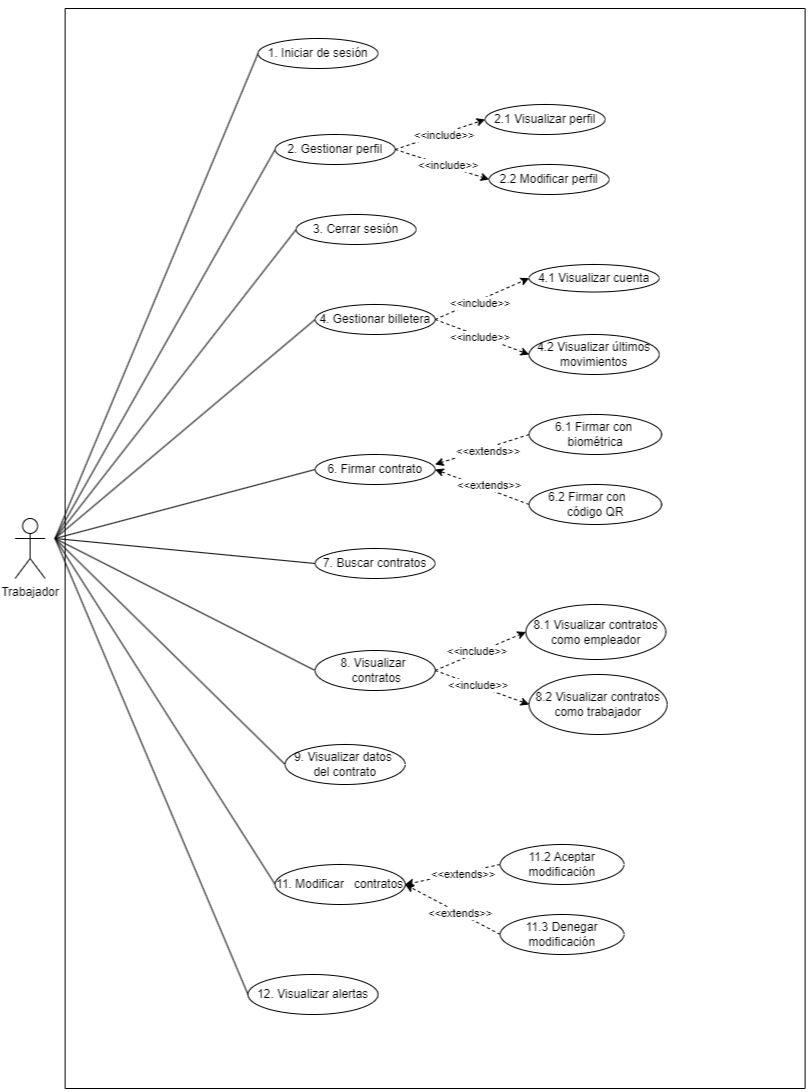
\includegraphics[width=\textwidth]{CasoUsoTrabajador}
	\caption[Diagrama de casos de uso trabajador]{Diagrama de casos de uso para el trabajador.}
\end{figure}


\begin{figure}[h]
	\label{img:CasoUsoEmpleador}
	\centering
	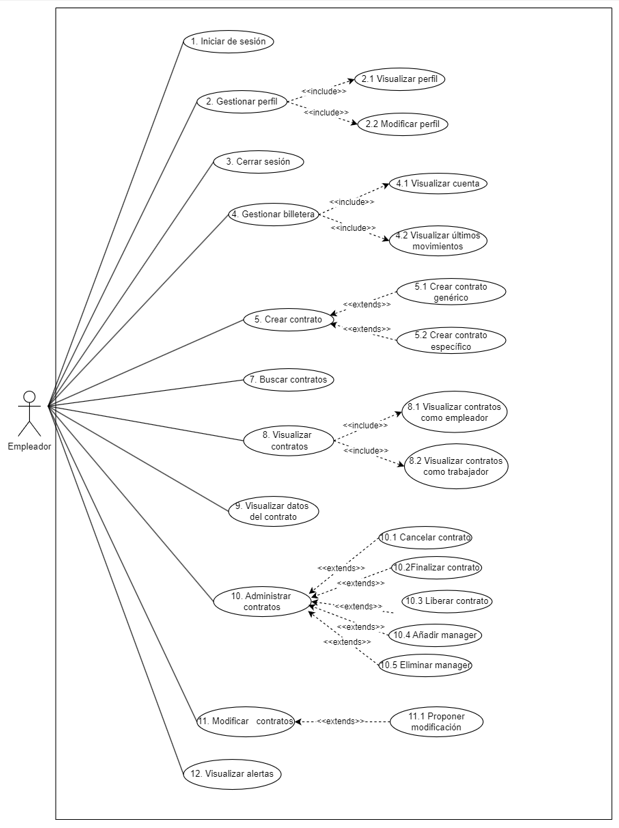
\includegraphics[width=\textwidth]{CasoUsoEmpleador}
	\caption[Diagrama de casos de uso empleador]{Diagrama de casos de uso para el empleador.}
\end{figure}



\begin{table}[p]
	\centering
	\begin{tabularx}{\linewidth}{ p{0.21\columnwidth} p{0.71\columnwidth} }
		\toprule
		\textbf{CU-1}    & \textbf{Iniciar sesión}\\
		\toprule
		\textbf{Versión}              & 1.0    \\
		\textbf{Autor}                & David Martínez Bahillo \\
		\textbf{Requisitos asociados} & RF-1.1 \\
		\textbf{Descripción}          & Permite al usuario acceder a su cuenta proporcionando sus credenciales de autenticación. \\
		\textbf{Precondición}         &  
		\begin{enumerate}
		\def\labelenumi{\arabic{enumi}.}
			\tightlist
			\item El usuario debe estar registrado.
			\item El usuario no debe tener una sesión activa.
		\end{enumerate}\\
		\textbf{Acciones}             &
		\begin{enumerate}
			\def\labelenumi{\arabic{enumi}.}
			\tightlist
			\item El usuario introduce su nombre de usuario y contraseña.
			\item El usuario selecciona la opción `Iniciar sesión'.
			\item El sistema verifica la información y concede el acceso si los datos son correctos.
		\end{enumerate}\\
		\textbf{Postcondición}        & El usuario accede a su cuenta y puede utilizar las funcionalidades del sistema. \\
		\textbf{Excepciones}          & Error al iniciar sesión. Por favor inténtelo de nuevo. \\
		\textbf{Importancia}          & Alta.  \\
		\bottomrule
	\end{tabularx}
	\caption{CU-1 Iniciar sesión.}
\end{table}




\begin{table}[p]
	\centering
	\begin{tabularx}{\linewidth}{ p{0.21\columnwidth} p{0.71\columnwidth} }
		\toprule
		\textbf{CU-2}    & \textbf{Gestionar perfil}\\
		\midrule
		\textbf{Versión}              & 1.0    \\
		\textbf{Autor}                & David Martínez Bahillo \\
		\textbf{Requisitos asociados} & RF-1.2, RF-1.3 \\
		\textbf{Descripción}          & Permite al usuario visualizar y modificar su perfil. \\
		\textbf{Precondición}         &  El usuario debe estar registrado y \textit{logueado}. \\
		\textbf{Acciones}             & El usuario selecciona `Ajustes'. \\
		\textbf{Postcondición}        & Se volverá a la pagina inicio tras completar la acción necesaria. \\
		\textbf{Excepciones}          & No se ha encontrado documento, Error al actualizar.  \\
		\textbf{Importancia}          & Baja.  \\
		\bottomrule
	\end{tabularx}
	\caption{CU-2 Gestionar perfil.}
\end{table}



\begin{table}[p]
	\centering
	\begin{tabularx}{\linewidth}{ p{0.21\columnwidth} p{0.71\columnwidth} }
		\toprule
		\textbf{CU-2.1}    & \textbf{Visualizar perfil}\\
		\midrule
		\textbf{Versión}              & 1.0    \\
		\textbf{Autor}                & David Martínez Bahillo \\
		\textbf{Requisitos asociados} & RF-1.2 \\
		\textbf{Descripción}          & Permite al usuario consultar los datos de su perfil en la plataforma. \\
		\textbf{Precondición}         & El usuario debe estar registrado y \textit{logueado}. \\
		\textbf{Acciones}             & El usuario selecciona `Perfil'. \\
		\textbf{Postcondición}        & Se volverá a la página de inicio tras consultar el perfil. \\
		\textbf{Excepciones}          & No se ha encontrado documento. \\
		\textbf{Importancia}          & Baja.  \\
		\bottomrule
	\end{tabularx}
	\caption{CU-2.1 Visualizar perfil.}
\end{table}



\begin{table}[p]
	\centering
	\begin{tabularx}{\linewidth}{ p{0.21\columnwidth} p{0.71\columnwidth} }
		\toprule
		\textbf{CU-2.2}    & \textbf{Modificar perfil}\\
		\midrule
		\textbf{Versión}              & 1.0    \\
		\textbf{Autor}                & David Martínez Bahillo \\
		\textbf{Requisitos asociados} & RF-1.3 \\
		\textbf{Descripción}          & Permite al usuario modificar los datos de su perfil. \\
		\textbf{Precondición}         & El usuario debe estar registrado y \textit{logueado}. \\
		\textbf{Acciones}             &
		\parbox[t]{\linewidth}{
			\begin{enumerate}
				\item El usuario selecciona la opción de `Modificar perfil'.
				\item El usuario edita la información deseada y confirma los cambios.
				\item El sistema valida y guarda los cambios.
			\end{enumerate}
		} \\
		\textbf{Postcondición}        & Los datos del perfil del usuario son actualizados. \\
		\textbf{Excepciones}          & Error al actualizar. \\
		\textbf{Importancia}          & Baja.  \\
		\bottomrule
	\end{tabularx}
	\caption{CU-2.2 Modificar perfil.}
\end{table}


\begin{table}[p]
	\centering
	\begin{tabularx}{\linewidth}{ p{0.21\columnwidth} p{0.71\columnwidth} }
		\toprule
		\textbf{CU-3}    & \textbf{Cerrar sesión}\\
		\midrule
		\textbf{Versión}              & 1.0    \\
		\textbf{Autor}                & David Martínez Bahillo \\
		\textbf{Requisitos asociados} & RF-1.4 \\
		\textbf{Descripción}          & Permite al usuario cerrar su sesión activa en la plataforma. \\
		\textbf{Precondición}         & El usuario debe estar registrado y \textit{logueado}. \\
		\textbf{Acciones}             &
		\begin{enumerate}
			\def\labelenumi{\arabic{enumi}.}
			\tightlist
			\item El usuario selecciona la opción `Cerrar sesión'.
			\item El sistema termina la sesión y redirige al usuario a la pantalla de inicio de sesión.
		\end{enumerate}\\
		\textbf{Postcondición}        & El usuario deja de estar \textit{logueado} en el sistema. \\
		\textbf{Excepciones}          & Error cerrando sesión. \\
		\textbf{Importancia}          & Media.  \\
		\bottomrule
	\end{tabularx}
	\caption{CU-3 Cerrar sesión.}
\end{table}


\begin{table}[p]
	\centering
	\begin{tabularx}{\linewidth}{ p{0.21\columnwidth} p{0.71\columnwidth} }
		\toprule
		\textbf{CU-4}    & \textbf{Gestionar billetera}\\
		\midrule
		\textbf{Versión}              & 1.0    \\
		\textbf{Autor}                & David Martínez Bahillo \\
		\textbf{Requisitos asociados} & RF-2.1, RF-2.2 \\
		\textbf{Descripción}          & Permite al usuario visualizar su cuenta y movimientos recientes. \\
		\textbf{Precondición}         &  El usuario debe estar registrado y \textit{logueado}. \\
		\textbf{Acciones}             &
		\begin{enumerate}
			\def\labelenumi{\arabic{enumi}.}
			\tightlist
			\item El usuario selecciona la opción `Cartera'.
			\item El sistema muestra las opciones de visualización de cuenta y movimientos.
		\end{enumerate}\\
		\textbf{Postcondición}        & El usuario visualiza la información de su billetera. \\
		\textbf{Excepciones}          & Error al obtener el historial de la cuenta. \\
		\textbf{Importancia}          & Media.  \\
		\bottomrule
	\end{tabularx}
	\caption{CU-4 Gestionar billetera.}
\end{table}


\begin{table}[p]
	\centering
	\begin{tabularx}{\linewidth}{ p{0.21\columnwidth} p{0.71\columnwidth} }
		\toprule
		\textbf{CU-4.1}  & \textbf{Visualizar cuenta}\\
		\midrule
		\textbf{Versión}              & 1.0    \\
		\textbf{Autor}                & David Martínez Bahillo \\
		\textbf{Requisitos asociados} & RF-2.1 \\
		\textbf{Descripción}          & Permite al usuario ver el la dirección y activos de su cuenta en la plataforma. \\
		\textbf{Precondición}         &  
		\begin{enumerate}
			\def\labelenumi{\arabic{enumi}.}
			\tightlist
			\item El usuario debe estar registrado y \textit{logueado}.
			\item El usuario ha seleccionado `Cartera'.
		\end{enumerate}\\
		\textbf{Acciones}             & El sistema muestra los detalles de la cuenta.\\
		\textbf{Postcondición}        & El usuario conoce el estado de su cuenta. \\
		\textbf{Excepciones}          & Ninguna. \\
		\textbf{Importancia}          & Media.  \\
		\bottomrule
	\end{tabularx}
	\caption{CU-4.1 Visualizar cuenta.}
\end{table}


\begin{table}[p]
	\centering
	\begin{tabularx}{\linewidth}{ p{0.21\columnwidth} p{0.71\columnwidth} }
		\toprule
		\textbf{CU-4.2}  & \textbf{Visualizar últimos movimientos}\\
		\midrule
		\textbf{Versión}              & 1.0    \\
		\textbf{Autor}                & David Martínez Bahillo \\
		\textbf{Requisitos asociados} & RF-2.2 \\
		\textbf{Descripción}          & Permite al usuario ver los últimos movimientos financieros en su cuenta. \\
		\textbf{Precondición}         &  
		\begin{enumerate}
			\def\labelenumi{\arabic{enumi}.}
			\tightlist
			\item El usuario debe estar registrado y \textit{logueado}.
			\item El usuario ha seleccionado `Cartera'.
		\end{enumerate}\\
		\textbf{Acciones}             & El sistema muestra la lista de movimientos recientes. \\
		\textbf{Postcondición}        & El usuario conoce sus últimos movimientos financieros. \\
		\textbf{Excepciones}          & Error al obtener el historial de la cuenta. \\
		\textbf{Importancia}          & Media.  \\
		\bottomrule
	\end{tabularx}
	\caption{CU-4.2 Visualizar últimos movimientos.}
\end{table}


\begin{table}[p]
	\centering
	\begin{tabularx}{\linewidth}{ p{0.21\columnwidth} p{0.71\columnwidth} }
		\toprule
		\textbf{CU-5}    & \textbf{Crear contrato}\\
		\midrule
		\textbf{Versión}              & 1.0    \\
		\textbf{Autor}                & David Martínez Bahillo \\
		\textbf{Requisitos asociados} & RF-3.1, RF-3.2 \\
		\textbf{Descripción}          & Permite al usuario iniciar el proceso de creación de un contrato, seleccionando entre un contrato genérico o específico. \\
		\textbf{Precondición}         &  
		\begin{enumerate}
			\def\labelenumi{\arabic{enumi}.}
			\tightlist
			\item El usuario debe estar registrado y \textit{logueado}.
			\item El usuario debe tener activos suficientes para crear el contrato.
		\end{enumerate}\\
		\textbf{Acciones}             &
		\begin{enumerate}
			\def\labelenumi{\arabic{enumi}.}
			\tightlist
			\item El usuario selecciona la opción `Crear contrato'.
			\item El usuario completa los campos necesarios y confirma la creación del contrato.
		\end{enumerate}\\
		\textbf{Postcondición}        & El usuario inicia el proceso de creación de un contrato. \\
		\textbf{Excepciones}          & Por favor, introduce todos los datos. La hora de inicio no puede ser
		 anterior a la hora actual. La fecha de finalización no puede ser anterior a la fecha de inicio.
		 Dirección de destinatario inválida. No puedes crear un contrato con tu propia dirección. Error al
		 crear el contrato.  \\
		\textbf{Importancia}          & Alta.  \\
		\bottomrule
	\end{tabularx}
	\caption{CU-5 Crear contrato.}
\end{table}


\begin{table}[p]
	\centering
	\begin{tabularx}{\linewidth}{ p{0.21\columnwidth} p{0.71\columnwidth} }
		\toprule
		\textbf{CU-5.1}  & \textbf{Crear contrato genérico}\\
		\midrule
		\textbf{Versión}              & 1.0    \\
		\textbf{Autor}                & David Martínez Bahillo \\
		\textbf{Requisitos asociados} & RF-3.1 \\
		\textbf{Descripción}          & Permite al usuario crear un contrato genérico con plantillas prediseñadas. \\
		\textbf{Precondición}         &  
		\begin{enumerate}
			\def\labelenumi{\arabic{enumi}.}
			\tightlist
			\item El usuario debe estar registrado y \textit{logueado}.
			\item El usuario debe tener activos suficientes para crear el contrato.
			\item El usuario no específica la cuenta del trabajador.
		\end{enumerate}\\
		\textbf{Acciones}             &
		\begin{enumerate}
			\def\labelenumi{\arabic{enumi}.}
			\tightlist
			\item El usuario selecciona la opción `Crear contrato'.
			\item El usuario completa los campos necesarios excepto el campo de `trabajador'.
			\item El usuario confirma la creación del contrato.
		\end{enumerate}\\
		\textbf{Postcondición}        & Se crea un nuevo contrato genérico según las especificaciones del usuario. \\
			\textbf{Excepciones}      & Por favor, introduce todos los datos. La hora de inicio no puede 
			ser anterior a la hora actual. La fecha de finalización no puede ser anterior a la fecha de
			inicio. Error al crear el contrato.  \\
		\textbf{Importancia}          & Alta.  \\
		\bottomrule
	\end{tabularx}
	\caption{CU-5.1 Crear contrato genérico.}
\end{table}


\begin{table}[p]
	\centering
	\begin{tabularx}{\linewidth}{ p{0.21\columnwidth} p{0.71\columnwidth} }
		\toprule
		\textbf{CU-5.2}  & \textbf{Crear contrato específico}\\
		\midrule
		\textbf{Versión}              & 1.0    \\
		\textbf{Autor}                & David Martínez Bahillo \\
		\textbf{Requisitos asociados} & RF-3.2 \\
		\textbf{Descripción}          & Permite al usuario crear un contrato personalizado, especificando todos los detalles necesarios. \\
		\textbf{Precondición}         &  
		\begin{enumerate}
			\def\labelenumi{\arabic{enumi}.}
			\tightlist
			\item El usuario debe estar registrado y \textit{logueado}.
			\item El usuario debe tener activos suficientes para crear el contrato.
			\item El usuario específica la cuenta del trabajador.
		\end{enumerate}\\
		\textbf{Acciones}             &
		\begin{enumerate}
			\def\labelenumi{\arabic{enumi}.}
			\tightlist
			\item El usuario selecciona la opción `Crear contrato'.
			\item El usuario completa los campos necesarios incluyendo el campo de `trabajador'.
			\item El usuario confirma la creación del contrato.
		\end{enumerate}\\
		\textbf{Postcondición}        & Se crea un nuevo contrato específico conforme a los requerimientos del
		 usuario. \\
		\textbf{Excepciones}          & Por favor, introduce todos los datos. La hora de inicio no puede ser
		 anterior a la hora actual. La fecha de finalización no puede ser anterior a la fecha de inicio.
		 Dirección de destinatario inválida. No puedes crear un contrato con tu propia dirección. Error al
		 crear el contrato.  \\
		\textbf{Importancia}          & Alta.  \\
		\bottomrule
	\end{tabularx}
	\caption{CU-5.2 Crear contrato específico.}
\end{table}


\begin{table}[p]
	\centering
	\begin{tabularx}{\linewidth}{ p{0.21\columnwidth} p{0.71\columnwidth} }
		\toprule
		\textbf{CU-6}    & \textbf{Firmar contrato}\\
		\midrule
		\textbf{Versión}              & 1.0    \\
		\textbf{Autor}                & David Martínez Bahillo \\
		\textbf{Requisitos asociados} & RF-4.1, RF-4.2 \\
		\textbf{Descripción}          & Permite al usuario firmar un contrato utilizando métodos biométricos o un código QR. \\
		\textbf{Precondición}         &  
		\begin{enumerate}
			\def\labelenumi{\arabic{enumi}.}
			\tightlist
			\item El usuario debe estar registrado y \textit{logueado}.
			\item El usuario ha seleccionado un contrato para firmar.
		\end{enumerate}\\
		\textbf{Acciones}             &
		\begin{enumerate}
			\def\labelenumi{\arabic{enumi}.}
			\tightlist
			\item El usuario elige el método de firma: biométrico o código QR.
			\item El sistema procesa la firma según el método seleccionado.
		\end{enumerate}\\
		\textbf{Postcondición}        & El contrato queda firmado por el usuario. \\
		\textbf{Excepciones}          & Error al firmar el contrato. El contrato no se ha podido firmar, 
		inténtalo de nuevo. \\
		\textbf{Importancia}          & Alta.  \\
		\bottomrule
	\end{tabularx}
	\caption{CU-6 Firmar contrato.}
\end{table}


\begin{table}[p]
	\centering
	\begin{tabularx}{\linewidth}{ p{0.21\columnwidth} p{0.71\columnwidth} }
		\toprule
		\textbf{CU-6.1}  & \textbf{Firmar con biométrica}\\
		\midrule
		\textbf{Versión}              & 1.0    \\
		\textbf{Autor}                & David Martínez Bahillo \\
		\textbf{Requisitos asociados} & RF-4.1 \\
		\textbf{Descripción}          & Permite al usuario firmar un contrato utilizando su identificación biométrica. \\
		\textbf{Precondición}         &  
		\begin{enumerate}
			\def\labelenumi{\arabic{enumi}.}
			\tightlist
			\item El usuario debe estar registrado y \textit{logueado}.
			\item El contrato debe estar listo para ser firmado.
		\end{enumerate}\\
		\textbf{Acciones}             &
		\begin{enumerate}
			\def\labelenumi{\arabic{enumi}.}
			\tightlist
			\item El usuario selecciona la opción de `firmar contrato'.
			\item El sistema verifica la identidad del usuario mediante el método biométrico elegido.
		\end{enumerate}\\
		\textbf{Postcondición}        & El contrato queda firmado mediante un método biométrico. \\
		\textbf{Excepciones}          & El contrato no se ha podido firmar, 
		inténtalo de nuevo. \\
		\textbf{Importancia}          & Alta.  \\
		\bottomrule
	\end{tabularx}
	\caption{CU-6.1 Firmar con biométrica.}
\end{table}


\begin{table}[p]
	\centering
	\begin{tabularx}{\linewidth}{ p{0.21\columnwidth} p{0.71\columnwidth} }
		\toprule
		\textbf{CU-6.2}  & \textbf{Firmar con código QR}\\
		\midrule
		\textbf{Versión}              & 1.0    \\
		\textbf{Autor}                & David Martínez Bahillo \\
		\textbf{Requisitos asociados} & RF-4.2 \\
		\textbf{Descripción}          & Permite al usuario firmar un contrato mediante la generación y escaneo de un código QR. \\
		\textbf{Precondición}         &  
		\begin{enumerate}
			\def\labelenumi{\arabic{enumi}.}
			\tightlist
			\item El usuario debe estar registrado y \textit{logueado}.
			\item El contrato debe estar listo para ser firmado.
		\end{enumerate}\\
		\textbf{Acciones}             &
		\begin{enumerate}
			\def\labelenumi{\arabic{enumi}.}
			\tightlist
			\item El usuario selecciona la opción `escanear código QR'.
			\item El sistema genera un código QR que el usuario debe escanear para confirmar la firma.
		\end{enumerate}\\
		\textbf{Postcondición}        & El contrato queda firmado mediante la validación del código QR. \\
		\textbf{Excepciones}          & El contrato no se ha podido firmar, 
		inténtalo de nuevo. \\
		\textbf{Importancia}          & Alta.  \\
		\bottomrule
	\end{tabularx}
	\caption{CU-6.2 Firmar con código QR.}
\end{table}


\begin{table}[p]
	\centering
	\begin{tabularx}{\linewidth}{ p{0.21\columnwidth} p{0.71\columnwidth} }
		\toprule
		\textbf{CU-7}    & \textbf{Buscar contratos}\\
		\midrule
		\textbf{Versión}              & 1.0    \\
		\textbf{Autor}                & David Martínez Bahillo \\
		\textbf{Requisitos asociados} & RF-5.1 \\
		\textbf{Descripción}          & Permite al usuario buscar contratos que se ofertan en la aplicación. \\
		\textbf{Precondición}         & El usuario debe estar registrado y \textit{logueado}. \\
		\textbf{Acciones}             &
		\begin{enumerate}
			\def\labelenumi{\arabic{enumi}.}
			\tightlist
			\item El usuario accede a `Buscar contratos'.
			\item El sistema muestra los contratos que coinciden con los criterios especificados.
		\end{enumerate}\\
		\textbf{Postcondición}        & El usuario visualiza la lista de contratos disponibles. \\
		\textbf{Excepciones}          & Error al obtener contratos sin firmar. \\
		\textbf{Importancia}          & Media. \\
		\bottomrule
	\end{tabularx}
	\caption{CU-7 Buscar contratos.}
\end{table}


\begin{table}[p]
	\centering
	\begin{tabularx}{\linewidth}{ p{0.21\columnwidth} p{0.71\columnwidth} }
		\toprule
		\textbf{CU-8}    & \textbf{Visualizar contratos}\\
		\midrule
		\textbf{Versión}              & 1.0    \\
		\textbf{Autor}                & David Martínez Bahillo \\
		\textbf{Requisitos asociados} & RF-6 \\
		\textbf{Descripción}          & Permite al usuario visualizar los contratos en los que el usuario esté involucrado. \\
		\textbf{Precondición}         &  
		\begin{enumerate}
			\def\labelenumi{\arabic{enumi}.}
			\tightlist
			\item El usuario debe estar registrado y \textit{logueado}.
			\item El usuario ha accedido a la pantalla `Mis Contratos'.
		\end{enumerate}\\
		\textbf{Acciones}             &
		\begin{enumerate}
			\def\labelenumi{\arabic{enumi}.}
			\tightlist
			\item El usuario accede a la pantalla `Mis contratos'.
			\item El sistema muestra todos los contratos en los que el usuario esté involucrado.
		\end{enumerate}\\
		\textbf{Postcondición}        & El usuario visualiza los contratos en los que esté involucrado. \\
		\textbf{Excepciones}          & Error al obtener los contratos. Error al cargar los contratos. \\
		\textbf{Importancia}          & Alta. \\
		\bottomrule
	\end{tabularx}
	\caption{CU-8 Visualizar contratos.}
\end{table}


\begin{table}[p]
	\centering
	\begin{tabularx}{\linewidth}{ p{0.21\columnwidth} p{0.71\columnwidth} }
		\toprule
		\textbf{CU-8.1}  & \textbf{Visualizar contratos como empleador}\\
		\midrule
		\textbf{Versión}              & 1.0    \\
		\textbf{Autor}                & David Martínez Bahillo \\
		\textbf{Requisitos asociados} & RF-6.1 \\
		\textbf{Descripción}          & Permite al usuario visualizar todos los contratos como empleador en los que se encuentre involucrado. \\
		\textbf{Precondición}         &  
		\begin{enumerate}
			\def\labelenumi{\arabic{enumi}.}
			\tightlist
			\item El usuario debe estar registrado y \textit{logueado}.
			\item El usuario a accedido a la pantalla `Mis Contratos'.
			\item El usuario a accedido a la sección `Mostrar contratos como empleador'.
		\end{enumerate}\\
		\textbf{Acciones}             &
		\begin{enumerate}
			\def\labelenumi{\arabic{enumi}.}
			\tightlist
			\item El usuario selecciona la opción de visualizar contratos como empleador.
			\item El sistema muestra la lista de contratos activos.
		\end{enumerate}\\
		\textbf{Postcondición}        & El usuario visualiza todos los contratos como empleador en la plataforma. \\
		\textbf{Excepciones}          & Error al obtener los contratos. Error al cargar los contratos. \\
		\textbf{Importancia}          & Alta. \\
		\bottomrule
	\end{tabularx}
	\caption{CU-8.1 Visualizar contratos como empleador.}
\end{table}


\begin{table}[p]
	\centering
	\begin{tabularx}{\linewidth}{ p{0.21\columnwidth} p{0.71\columnwidth} }
		\toprule
		\textbf{CU-8.1}  & \textbf{Visualizar contratos como trabajador}\\
		\midrule
		\textbf{Versión}              & 1.0    \\
		\textbf{Autor}                & David Martínez Bahillo \\
		\textbf{Requisitos asociados} & RF-6.2 \\
		\textbf{Descripción}          & Permite al usuario visualizar todos los contratos como empleador en los que se encuentre involucrado. \\
		\textbf{Precondición}         &  
		\begin{enumerate}
			\def\labelenumi{\arabic{enumi}.}
			\tightlist
			\item El usuario debe estar registrado y \textit{logueado}.
			\item El usuario a accedido a la pantalla `Mis Contratos'.
			\item El usuario a accedido a la sección `Mostrar contratos como trabajador'.
		\end{enumerate}\\
		\textbf{Acciones}             &
		\begin{enumerate}
			\def\labelenumi{\arabic{enumi}.}
			\tightlist
			\item El usuario selecciona la opción de visualizar contratos como trabajador.
			\item El sistema muestra la lista de contratos activos.
		\end{enumerate}\\
		\textbf{Postcondición}        & El usuario visualiza todos los contratos como trabajador en la plataforma. \\
		\textbf{Excepciones}          & Error al obtener los contratos. Error al cargar los contratos. \\
		\textbf{Importancia}          & Alta. \\
		\bottomrule
	\end{tabularx}
	\caption{CU-8.2 Visualizar contratos como trabajador.}
\end{table}


\begin{table}[p]
	\centering
	\begin{tabularx}{\linewidth}{ p{0.21\columnwidth} p{0.71\columnwidth} }
		\toprule
		\textbf{CU-9}    & \textbf{Administrar contratos}\\
		\midrule
		\textbf{Versión}              & 1.0    \\
		\textbf{Autor}                & David Martínez Bahillo \\
		\textbf{Requisitos asociados} & RF-8 \\
		\textbf{Descripción}          & Permite al usuario gestionar activamente sus contratos, incluyendo cancelación, finalización, liberación de pagos y gestión de managers. \\
		\textbf{Precondición}         & El usuario debe estar registrado y \textit{logueado}. \\
		\textbf{Acciones}             & El usuario se encuentra en la pantalla de detalles del contrato. \\
		\textbf{Postcondición}        & El usuario gestiona sus contratos de acuerdo a sus necesidades. \\
		\textbf{Excepciones}          & Error al finalizar el contrato. Error al cancelar el contrato. Error al
		 liberar el salario. Error al asignar manager. Error al eliminar manager. \\
		\textbf{Importancia}          & Alta. \\
		\bottomrule
	\end{tabularx}
	\caption{CU-9 Administrar contratos.}
\end{table}


\begin{table}[p]
	\centering
	\begin{tabularx}{\linewidth}{ p{0.21\columnwidth} p{0.71\columnwidth} }
		\toprule
		\textbf{CU-9.1}  & \textbf{Cancelar contrato}\\
		\midrule
		\textbf{Versión}              & 1.0    \\
		\textbf{Autor}                & David Martínez Bahillo \\
		\textbf{Requisitos asociados} & RF-8.1 \\
		\textbf{Descripción}          & Permite al usuario cancelar un contrato antes de que se firme. \\
		\textbf{Precondición}         &  
		\begin{enumerate}
			\item El usuario debe estar registrado y \textit{logueado}.
			\item El contrato debe estar en estado de pendiente de firma.
		\end{enumerate}\\
		\textbf{Acciones}             &
		\begin{enumerate}
			\item El usuario selecciona la opción `Cancelar contrato'.
			\item El sistema confirma la cancelación del contrato.
		\end{enumerate}\\
		\textbf{Postcondición}        & El contrato queda cancelado y no es vinculante para ninguna de las partes. \\
		\textbf{Excepciones}          & Error al cancelar el contrato. \\
		\textbf{Importancia}          & Media. \\
		\bottomrule
	\end{tabularx}
	\caption{CU-9.1 Cancelar contrato.}
\end{table}


\begin{table}[p]
	\centering
	\begin{tabularx}{\linewidth}{ p{0.21\columnwidth} p{0.71\columnwidth} }
		\toprule
		\textbf{CU-9.2}  & \textbf{Finalizar contrato}\\
		\midrule
		\textbf{Versión}              & 1.0    \\
		\textbf{Autor}                & David Martínez Bahillo \\
		\textbf{Requisitos asociados} & RF-8.2 \\
		\textbf{Descripción}          & Permite al usuario finalizar un contrato de manera formal una vez que se hayan cumplido los términos acordados. \\
		\textbf{Precondición}         &  
		\begin{enumerate}
			\item El usuario debe estar registrado y \textit{logueado}.
			\item Los términos del contrato deben estar cumplidos.
		\end{enumerate}\\
		\textbf{Acciones}             &
		\begin{enumerate}
			\item El usuario selecciona la opción `Finalizar contrato'.
			\item El sistema confirma la finalización del contrato.
		\end{enumerate}\\
		\textbf{Postcondición}        & El contrato queda formalmente finalizado. \\
		\textbf{Excepciones}          & Error al finalizar el contrato. \\
		\textbf{Importancia}          & Alta. \\
		\bottomrule
	\end{tabularx}
	\caption{CU-9.2 Finalizar contrato.}
\end{table}


\begin{table}[p]
	\centering
	\begin{tabularx}{\linewidth}{ p{0.21\columnwidth} p{0.71\columnwidth} }
		\toprule
		\textbf{CU-9.3}  & \textbf{Liberar contrato}\\
		\midrule
		\textbf{Versión}              & 1.0    \\
		\textbf{Autor}                & David Martínez Bahillo \\
		\textbf{Requisitos asociados} & RF-8.3 \\
		\textbf{Descripción}          & Permite al empleador liberar y transferir los fondos acordados una vez cumplidos los términos del contrato. \\
		\textbf{Precondición}         &  
		\begin{enumerate}
			\item El usuario debe estar registrado y \textit{logueado}.
			\item El contrato debe estar finalizado.
		\end{enumerate}\\
		\textbf{Acciones}             &
		\begin{enumerate}
			\item El usuario selecciona la opción `Liberar salario'.
			\item El sistema procesa la liberación y transferencia de los fondos al trabajador.
		\end{enumerate}\\
		\textbf{Postcondición}        & Los fondos son transferidos según los términos del contrato. \\
		\textbf{Excepciones}          & Error al liberar el salario. \\
		\textbf{Importancia}          & Alta. \\
		\bottomrule
	\end{tabularx}
	\caption{CU-9.3 Liberar contrato.}
\end{table}


\begin{table}[p]
	\centering
	\begin{tabularx}{\linewidth}{ p{0.21\columnwidth} p{0.71\columnwidth} }
		\toprule
		\textbf{CU-9.4}  & \textbf{Añadir manager}\\
		\midrule
		\textbf{Versión}              & 1.0    \\
		\textbf{Autor}                & David Martínez Bahillo \\
		\textbf{Requisitos asociados} & RF-8.4 \\
		\textbf{Descripción}          & Permite al usuario agregar un nuevo manager para la gestión del contrato. \\
		\textbf{Precondición}         &  
		\begin{enumerate}
			\item El usuario debe estar registrado y \textit{logueado}.
			\item El contrato debe estar activo.
			\item El manager no puede ser el propio trabajador.
		\end{enumerate}\\
		\textbf{Acciones}             &
		\begin{enumerate}
			\item El usuario selecciona la opción `Añadir manager'.
			\item El usuario ingresa los datos del nuevo manager.
			\item El sistema confirma la adición del nuevo manager.
		\end{enumerate}\\
		\textbf{Postcondición}        & El nuevo manager es añadido al contrato. \\
		\textbf{Excepciones}          & Error al asignar manager. \\
		\textbf{Importancia}          & Media. \\
		\bottomrule
	\end{tabularx}
	\caption{CU-9.4 Añadir manager.}
\end{table}


\begin{table}[p]
	\centering
	\begin{tabularx}{\linewidth}{ p{0.21\columnwidth} p{0.71\columnwidth} }
		\toprule
		\textbf{CU-9.5}  & \textbf{Eliminar manager}\\
		\midrule
		\textbf{Versión}              & 1.0    \\
		\textbf{Autor}                & David Martínez Bahillo \\
		\textbf{Requisitos asociados} & RF-8.5 \\
		\textbf{Descripción}          & Permite al usuario eliminar un manager actualmente asignado al contrato. \\
		\textbf{Precondición}         &  
		\begin{enumerate}
			\item El usuario debe estar registrado y \textit{logueado}.
			\item El contrato debe estar activo.
			\item El manager debe de estar asignado previamente a dicho contrato.
		\end{enumerate}\\
		\textbf{Acciones}             &
		\begin{enumerate}
			\item El usuario selecciona elimina al manager.
			\item El sistema confirma la eliminación del manager.
		\end{enumerate}\\
		\textbf{Postcondición}        & El manager es eliminado del contrato. \\
		\textbf{Excepciones}          & Error al eliminar manager. \\
		\textbf{Importancia}          & Media. \\
		\bottomrule
	\end{tabularx}
	\caption{CU-9.5 Eliminar manager.}
\end{table}


\begin{table}[p]
	\centering
	\begin{tabularx}{\linewidth}{ p{0.21\columnwidth} p{0.71\columnwidth} }
		\toprule
		\textbf{CU-10}    & \textbf{Modificar contratos}\\
		\midrule
		\textbf{Versión}              & 1.0    \\
		\textbf{Autor}                & David Martínez Bahillo \\
		\textbf{Requisitos asociados} & RF-9 \\
		\textbf{Descripción}          & Permite al usuario proponer, aceptar o denegar modificaciones a los contratos existentes. \\
				\textbf{Precondición}         &  
		\begin{enumerate}
			\item El usuario debe estar registrado y \textit{logueado}.
			\item El contrato debe estar activo.
		\end{enumerate}\\
		\textbf{Acciones}             & El usuario selecciona la opción `Modificar contratos'. \\
		\textbf{Postcondición}        & El usuario gestiona las modificaciones de sus contratos. \\
		\textbf{Excepciones}          & La fecha de finalización no puede ser anterior a la fecha de inicio. La fecha de finalización no puede ser anterior a la fecha actual. Error al modificar el contrato. Error al rechazar los cambios. Error al aceptar los cambios. \\
		\textbf{Importancia}          & Alta. \\
		\bottomrule
	\end{tabularx}
	\caption{CU-10 Modificar contratos.}
\end{table}


\begin{table}[p]
	\centering
	\begin{tabularx}{\linewidth}{ p{0.21\columnwidth} p{0.71\columnwidth} }
		\toprule
		\textbf{CU-10.1}  & \textbf{Proponer modificación}\\
		\midrule
		\textbf{Versión}              & 1.0    \\
		\textbf{Autor}                & David Martínez Bahillo \\
		\textbf{Requisitos asociados} & RF-9.1 \\
		\textbf{Descripción}          & Permite al usuario proponer modificaciones a los contratos existentes. \\
		\textbf{Precondición}         &  
		\begin{enumerate}
			\item El usuario debe estar registrado y \textit{logueado}.
			\item El contrato debe estar activo.
		\end{enumerate}\\
		\textbf{Acciones}             &
		\begin{enumerate}
			\item El usuario selecciona la opción `Modificar contrato'.
			\item El usuario introduce los cambios propuestos.
			\item El sistema guarda y notifica la propuesta de modificación a la otra parte.
		\end{enumerate}\\
		\textbf{Postcondición}        & La propuesta de modificación queda registrada y pendiente de aceptación o rechazo. \\
		\textbf{Excepciones}          & La fecha de finalización no puede ser anterior a la fecha de inicio. La fecha de finalización no puede ser anterior a la fecha actual. Error al modificar el contrato. \\
		\textbf{Importancia}          & Alta. \\
		\bottomrule
	\end{tabularx}
	\caption{CU-10.1 Proponer modificación.}
\end{table}


\begin{table}[p]
	\centering
	\begin{tabularx}{\linewidth}{ p{0.21\columnwidth} p{0.71\columnwidth} }
		\toprule
		\textbf{CU-10.2}  & \textbf{Aceptar modificación}\\
		\midrule
		\textbf{Versión}              & 1.0    \\
		\textbf{Autor}                & David Martínez Bahillo \\
		\textbf{Requisitos asociados} & RF-9.2 \\
		\textbf{Descripción}          & Permite al usuario aceptar las modificaciones propuestas a un contrato. \\
		\textbf{Precondición}         &  
		\begin{enumerate}
			\item El usuario debe estar registrado y \textit{logueado}.
			\item El contrato debe estar activo.
			\item Existe una propuesta de modificación pendiente.
		\end{enumerate}\\
		\textbf{Acciones}             &
		\begin{enumerate}
			\item El usuario selecciona la opción `Aceptar modificación'.
			\item El sistema actualiza el contrato con las modificaciones aceptadas.
		\end{enumerate}\\
		\textbf{Postcondición}        & El contrato se actualiza con las modificaciones aceptadas. \\
		\textbf{Excepciones}          & Error al aceptar los cambios. \\
		\textbf{Importancia}          & Alta. \\
		\bottomrule
	\end{tabularx}
	\caption{CU-10.2 Aceptar modificación.}
\end{table}


\begin{table}[p]
	\centering
	\begin{tabularx}{\linewidth}{ p{0.21\columnwidth} p{0.71\columnwidth} }
		\toprule
		\textbf{CU-10.3}  & \textbf{Denegar modificación}\\
		\midrule
		\textbf{Versión}              & 1.0    \\
		\textbf{Autor}                & David Martínez Bahillo \\
		\textbf{Requisitos asociados} & RF-9.3 \\
		\textbf{Descripción}          & Permite al usuario denegar las modificaciones propuestas a un contrato. \\
		\textbf{Precondición}         &  
		\begin{enumerate}
			\item El usuario debe estar registrado y \textit{logueado}.
			\item El contrato debe estar activo.
			\item Existe una propuesta de modificación pendiente.
		\end{enumerate}\\
		\textbf{Acciones}             &
		\begin{enumerate}
			\item El usuario selecciona la opción `Denegar modificación'.
			\item El sistema registra la denegación y notifica a la otra parte.
		\end{enumerate}\\
		\textbf{Postcondición}        & La propuesta de modificación queda denegada y el contrato permanece sin cambios. \\
		\textbf{Excepciones}          & Error al rechazar los cambios. \\
		\textbf{Importancia}          & Alta. \\
		\bottomrule
	\end{tabularx}
	\caption{CU-10.3 Denegar modificación.}
\end{table}


\begin{table}[p]
	\centering
	\begin{tabularx}{\linewidth}{ p{0.21\columnwidth} p{0.71\columnwidth} }
		\toprule
		\textbf{CU-11}    & \textbf{Visualizar alertas}\\
		\midrule
		\textbf{Versión}              & 1.0    \\
		\textbf{Autor}                & David Martínez Bahillo \\
		\textbf{Requisitos asociados} & RF-10 \\
		\textbf{Descripción}          & Permite al usuario visualizar las alertas y notificaciones relacionadas con sus contratos y actividades en la plataforma. \\
		\textbf{Precondición}         & El usuario debe estar registrado y \textit{logueado}. \\
		\textbf{Acciones}             &
		\begin{enumerate}
			\item El usuario accede a la sección de `Alertas'.
			\item El sistema muestra las alertas y notificaciones relevantes.
		\end{enumerate}\\
		\textbf{Postcondición}        & El usuario visualiza las alertas y notificaciones. \\
		\textbf{Excepciones}          & Error al obtener el historial de la cuenta. \\
		\textbf{Importancia}          & Media. \\
		\bottomrule
	\end{tabularx}
	\caption{CU-11 Visualizar alertas.}
\end{table}


\begin{table}[p]
	\centering
	\begin{tabularx}{\linewidth}{ p{0.21\columnwidth} p{0.71\columnwidth} }
		\toprule
		\textbf{CU-12}    & \textbf{Utilizar herramientas}\\
		\midrule
		\textbf{Versión}              & 1.0    \\
		\textbf{Autor}                & David Martínez Bahillo \\
		\textbf{Requisitos asociados} & RF-11 \\
		\textbf{Descripción}          & Permite al usuario acceder y utilizar diversas herramientas adicionales proporcionadas por la plataforma. \\
		\textbf{Precondición}         & El usuario debe estar registrado y \textit{logueado}. \\
		\textbf{Acciones}             & El usuario selecciona la opción `información'. \\
		\textbf{Postcondición}        & El usuario accede a las herramientas disponibles en la plataforma. \\
		\textbf{Excepciones}          & Ninguna. \\
		\textbf{Importancia}          & Baja. \\
		\bottomrule
	\end{tabularx}
	\caption{CU-12 Utilizar herramientas.}
\end{table}


\begin{table}[p]
	\centering
	\begin{tabularx}{\linewidth}{ p{0.21\columnwidth} p{0.71\columnwidth} }
		\toprule
		\textbf{CU-12.1}  & \textbf{Consultar información Ethereum}\\
		\midrule
		\textbf{Versión}              & 1.0    \\
		\textbf{Autor}                & David Martínez Bahillo \\
		\textbf{Requisitos asociados} & RF-11.1 \\
		\textbf{Descripción}          & Permite al usuario consultar la información actual y el histórico del precio de Ethereum. \\
		\textbf{Precondición}         &  
		\begin{enumerate}
			\item El usuario debe estar registrado y \textit{logueado}.
			\item El usuario ha seleccionado `información'.
		\end{enumerate}\\
		\textbf{Acciones}             &
		\begin{enumerate}
			\item El sistema muestra el precio actual y el histórico del Ethereum.
		\end{enumerate}\\
		\textbf{Postcondición}        & El usuario visualiza la información actual y el histórico del precio de Ethereum. \\
		\textbf{Excepciones}          & Ninguna. \\
		\textbf{Importancia}          & Baja. \\
		\bottomrule
	\end{tabularx}
	\caption{CU-12.1 Consultar información Ethereum.}
\end{table}


\begin{table}[p]
	\centering
	\begin{tabularx}{\linewidth}{ p{0.21\columnwidth} p{0.71\columnwidth} }
		\toprule
		\textbf{CU-12.2}  & \textbf{Usar calculadora de divisas}\\
		\midrule
		\textbf{Versión}              & 1.0    \\
		\textbf{Autor}                & David Martínez Bahillo \\
		\textbf{Requisitos asociados} & RF-11.2 \\
		\textbf{Descripción}          & Permite al usuario utilizar una calculadora para convertir entre Ethereum y euros, y viceversa. \\
		\textbf{Precondición}         &  
		\begin{enumerate}
			\item El usuario debe estar registrado y \textit{logueado}.
			\item El usuario ha seleccionado `información'.
		\end{enumerate}\\
		\textbf{Acciones}             &
		\begin{enumerate}
			\item El usuario introduce la cantidad a convertir y selecciona la divisa de destino.
			\item El sistema muestra el resultado de la conversión.
		\end{enumerate}\\
		\textbf{Postcondición}        & El usuario obtiene la conversión de la cantidad introducida entre Ethereum y euros. \\
		\textbf{Excepciones}          & Fallos en la actualización de los tipos de cambio. \\
		\textbf{Importancia}          & Baja. \\
		\bottomrule
	\end{tabularx}
	\caption{CU-12.2 Usar calculadora de divisas.}
\end{table}